\RequirePackage[T1]{fontenc}
\documentclass[journal,10pt]{IEEEtran}
\usepackage{mathptmx}
\usepackage{amsmath,amssymb,booktabs,array,multirow}
\usepackage{graphicx,xcolor}
\usepackage{placeins}
\usepackage{cite,url}
\usepackage[hidelinks]{hyperref}
\usepackage{tikz}
\usetikzlibrary{arrows.meta,positioning,fit,calc}
\newcommand{\LEAF}{\textsc{LEAF}}
\hyphenation{multi-agent gene-ra-li-za-tion re-pre-sen-ta-tion}
\hypersetup{pdftitle={LEAF: Reusable Threat Context for Zero-Shot Multi-Target Defense},pdfauthor={}}
\begin{document}
\raggedbottom
\title{LEAF: Reusable Threat Context for Zero-Shot Multi-Target Defense}
\author{Anonymous Authors}
\bstctlcite{leafBibliographyControl}
\maketitle
\markboth{Anonymous Manuscript Submitted for Review}{LEAF: Reusable Threat Context for Multi-Target Defense}
\begin{abstract}
In multi-target defense, deployment populations often differ from those seen during training. Variable-size entity inputs accommodate this change, but effective protection also requires interpreting an attacker together with the target it approaches and the teammates already covering that target. We propose Looped Entity Attention Fusion (LEAF), which constructs this threat context through a shared iterative attention operator. Training samples the refinement depth and fuses intermediate reads. Each defender queries the context using its current self representation, while recurrent memory enters downstream. In SkyHAD, policies trained with at most ten vehicles per team and three targets transfer without retraining to fifty vehicles per team or twelve targets. Across three training seeds, LEAF reduces mean target damage relative to REFIL by 0.800, 1.635, and 2.211 in target-count, team-size, and joint extrapolation, respectively, and leads all compared learned baselines in each group. Historical design comparisons favor current-state reading, while frozen interventions show dependence on constructed context and downstream memory. Frozen execution from one to six rounds, including depths beyond training, preserves similar aggregate protection; normal reads place approximately 99\% of fusion weight on the first two stages. Permutation analysis and a finite-depth action-stability bound clarify the architecture's structural support. Together, the results connect reusable current-scene processing to population transfer, higher interception, and lower target-damage incidence.
\end{abstract}
\noindent\textbf{Note to Practitioners---}
A protection controller may face different numbers of vehicles and assets at deployment. LEAF trains a shared policy on small engagements and reuses its parameters on larger entity sets. Its current-scene encoder and downstream recurrent policy separate scene interpretation from temporal inference. The experiments measure accumulated target damage, interception, and friendly-collision mortality. They use a planar simulation with public entity-state observations and a fixed reactive attacker, so the results establish transfer under this interface. Execution depth is an externally selected budget; learned stage fusion combines information and does not stop computation automatically.
\par
\begin{IEEEkeywords}
Multi-agent reinforcement learning, population generalization, entity attention, target protection, iterative refinement.
\end{IEEEkeywords}
\section{Introduction}
\IEEEPARstart{M}{ulti-target} defense requires a team to protect several assets while the numbers of available defenders and incoming attackers change. A policy trained separately for every deployment population would be costly to maintain. The desired alternative is to train once on small engagements and reuse the same parameters when the team or the set of protected assets grows. Accepting a variable-size observation is necessary for this transfer, but the harder question is what information the policy should extract from that observation.

An attacker's threat is contextual. Its motion matters together with the asset it approaches and the teammates already covering that asset. We call this joint attacker--target--teammate information the \emph{threat context}. Figure~\ref{fig:motivation} illustrates two scenes with the same attacker--target approach geometry. In one, teammates already cover the target; in the other, the acting defender must respond to a coverage gap. The attacker alone does not distinguish these situations. A useful representation should combine target coverage with the approaching threat before the acting defender compresses the scene into its decision feature. With more entities, these relationships occur in new combinations, so the process that constructs the context must be reusable.

\begin{figure*}[!t]
\centering
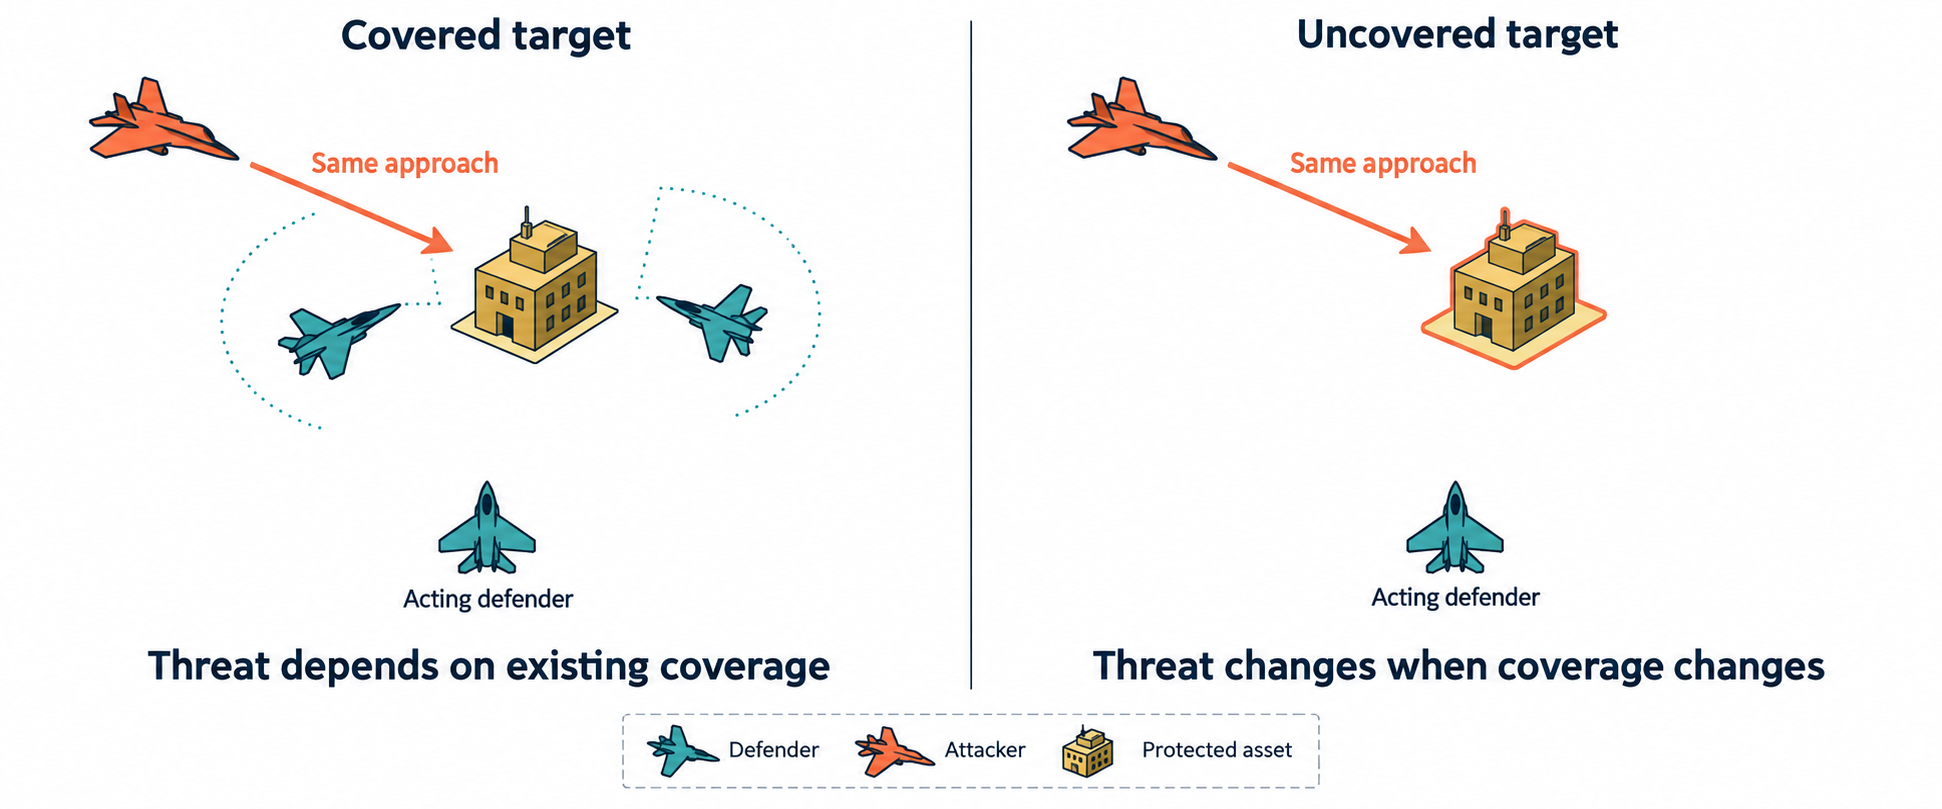
\includegraphics[width=0.92\textwidth]{figures/fig_motivation.png}
\caption{Motivation: matched attacker--target approach geometry can demand a different defensive response when teammate coverage changes. LEAF is designed to build this threat context before receiver-specific reading. The illustration is conceptual; coverage arcs are illustrative and are not simulator measurements.}
\label{fig:motivation}
\end{figure*}

Two further requirements shape the representation. First, the same scene has different implications for a free defender and one already engaged elsewhere. Reading should therefore be conditioned on the acting defender. Second, current scene processing and temporal inference have distinct roles. Attacker intent is not directly observed, so history remains useful for action selection. Yet a recurrent summary learned on small engagements may change distribution as the population grows. Feeding that summary back into every context read exposes scene interpretation to an additional source of shift. This motivates constructing and reading the current context before incorporating recurrent memory.

Existing approaches address parts of this problem. Differential games and task allocation organize interception through geometry, matching, and assignments~\cite{chen2017reachavoid,yan2020barriers,shishika2020perimeter}. Their guarantees rely on the chosen dynamics and task structure. Entity-based cooperative learning supports variable populations~\cite{iqbal2021refil,park2026spectra}, but a single self-to-entity attention read has no explicit intermediate stage for constructing the threat context. Hierarchical allocation, as in ALMA~\cite{iqbal2022alma}, introduces a discrete task organization before maneuvering. Entity Transformers such as UPDeT and TransfQMix~\cite{hu2021updet,transfqmix2023} perform richer interaction and incorporate temporal tokens. Their usual fixed-depth computation does not directly address how one current-scene refinement operator can be reused at different execution depths. Our focus is this organization of context construction, receiver-specific access, and memory.

We propose \textbf{Looped Entity Attention Fusion (LEAF)}. At each physical decision, a shared entity-attention operator repeatedly refines the current entity set. A query derived from the defender's current self representation reads each stage, and learned weights fuse the reads. Training samples the number of rounds, encouraging the same operator to support decisions at several exits. The fused context augments the REFIL feature, after which a temporal GRU incorporates history and produces action values. Parameters are shared across entities, defenders, and refinement rounds. The loop processes one observation; the GRU carries information between observations.

We evaluate frozen policies in SkyHAD after training only with at most ten vehicles per team and three targets. Deployment reaches fifty vehicles per team or twelve targets, with separate target-count, team-size, and joint extrapolation groups. LEAF has lower mean target damage than all compared learned baselines and the rule-based controller in each group. The experiments then distinguish three questions: whether the overall policy transfers, which design changes affect transfer, and how the frozen policy uses its refinement stages. The one-round exit of a multi-depth-trained LEAF remains effective even though a separately trained one-round model transfers less well on average. Execution through six rounds, beyond the training maximum of four, gives similar aggregate damage. These observations support reusable refinement over the evaluated range without assuming that more computation must always help.

Our contributions are:
\begin{enumerate}
\item A threat-context encoder combining shared iterative entity updates, current-state receiver queries, and stage fusion before temporal memory, integrated with cooperative value learning.
\item Structural analysis of permutation consistency and a finite-depth action-stability bound, clarifying what the architecture guarantees and what remains an empirical generalization claim.
\item A unified experimental account comprising baseline comparisons, seven trained design variants, and frozen-policy mechanism studies, connecting population transfer to depth robustness, intermediate reading, and target-protection behavior.
\end{enumerate}

\section{Related Work}
\subsection{Target Defense and Task Allocation}
Differential-game formulations describe interception and protection through feedback strategies, winning regions, and geometric barriers~\cite{garcia2019activedefense,chen2017reachavoid,yan2020barriers}. Matching combines subgame outcomes into team assignments, including heterogeneous three-dimensional reach--avoid problems~\cite{yan2022matching}. Cooperative perimeter defense likewise shows that a team's ability to stop an intruder depends on the joint defender arrangement~\cite{shishika2020perimeter}. These results motivate relational reasoning but obtain their guarantees under specified dynamics and geometry.

Multi-robot task allocation makes the distribution of effort explicit~\cite{gerkey2004allocation,choi2009auction}. Coalition auctions and integrated allocation--motion methods handle cooperative assignments and safe coordination~\cite{deng2024coalitions,miele2025coordination}. Learning-based hierarchies also organize swarm confrontation and target defense through allocation and execution~\cite{wu2025swarm,li2025targetdefense}. ALMA learns hierarchical allocation for composite multi-agent tasks~\cite{iqbal2022alma}. An assignment is a useful coordination abstraction, but it differs from maintaining an entity-level threat context that each defender can read before choosing its next maneuver. LEAF uses the latter organization without an explicit assignment output.

\subsection{Entity-Based Cooperative Learning}
Deep Sets, Set Transformers, and swarm mean embeddings support shared computation over variable-size collections~\cite{zaheer2017deepsets,lee2019settransformer,huttenrauch2019swarm}. Cooperative value decomposition, monotonic mixing, and coordination graphs connect individual utilities to team objectives~\cite{sunehag2018vdn,rashid2018qmix,boehmer2020dcg}. REFIL trains an auxiliary randomly factorized value function over entity groups to encourage transfer of reusable interactions~\cite{iqbal2021refil}; LEAF retains this host objective.

Representation choices remain distinct within this family. REFIL's attention feature and SPECTra's self-query aggregation~\cite{park2026spectra} read entities from an agent's perspective. UPDeT and TransfQMix use Transformer-based entity processing, with recurrent tokens carrying history~\cite{hu2021updet,transfqmix2023}. These architectures demonstrate that richer entity processing can support cooperative transfer. Our comparison asks whether organizing processing into a shared current-scene loop, fixed-self intermediate reading, and downstream recurrence improves multi-target protection. The evaluated baselines are their documented adaptations to the common maneuver task, while the LEAF variants provide closer architectural controls.

\subsection{Iterative Refinement and Intermediate Reading}
Relational reinforcement learning uses attention to model interactions among entities~\cite{zambaldi2019relational}. Universal Transformers share a transition across depth~\cite{dehghani2019universal}; Jumping Knowledge combines intermediate graph representations~\cite{xu2018jk}; LayerDrop trains computation paths of varying depth~\cite{fan2020layerdrop}. These ideas motivate reusable refinement and access to multiple stages, but do not establish reward improvements or convergence for a defense policy.

Temporal information remains essential under partial observability, including in attention-based multi-agent recurrence~\cite{phan2023aerial}. LEAF retains temporal recurrence while removing the recurrent hidden state from current-scene context construction and reading. Its contribution is the joint organization of these components around the threat-context problem, together with experiments separating population transfer, trained design changes, and frozen-depth behavior. The theoretical analysis concerns permutation consistency and a sufficient local condition for preserving actions across exits, rather than an unconditional scale-generalization guarantee.

\section{Problem Formulation and Preliminaries}
\label{sec:problem}
\subsection{Cooperative Target Protection}
We study cooperative target protection in the planar target-protection model of SkyHAD~\cite{skyhad2026} in which defenders coordinate their actions against incoming attackers across a changing set of protected targets. Let $\mathcal R$, $\mathcal B$, and $\mathcal T$ denote the defender, attacker, and target sets, with initial configuration $\mathbf n=(N_R,N_B,K)$. Targets occupy the left portion of the arena; attackers approach from the right, and defenders distribute their responses between interception and target coverage. Population transfer changes the sizes of these sets while preserving the interaction rules.

Vehicles choose among eight normalized acceleration directions and zero acceleration. Close vehicle encounters can remove both participants, while automatic firing allows defenders to engage attackers and attackers to damage targets. Targets remain as damage accumulates. The simulator continues after the final defender disappears and ends when all attackers have disappeared or the episode horizon is reached. Table~\ref{tab:environment} collects the physical interface used by all policies.

\begin{table}[t]
\centering\footnotesize
\caption{SkyHAD planar target-protection interface.}
\label{tab:environment}
\begin{tabular}{@{}ll@{}}\toprule
Quantity & Setting\\\midrule
Arena & $5000\times5000$ m\\
Decision interval / horizon & 1 s / 100 steps\\
Acceleration limit & $40\,\mathrm{m/s^2}$\\
Vehicle speed range & $35$--$120\,\mathrm{m/s}$\\
Swept collision distance & 20 m\\
Automatic firing separation & Below 200 m, pre-movement\\
Damage profile & Unit core to 200 m; linear to 0 at 400 m\\
\bottomrule\end{tabular}
\end{table}

Public observations contain entity positions, velocities, types, health or alive status, and target damage. The fixed reactive attacker controller selects a target using public defender coverage and distances, then carries out a rush and periodically revises its assignment. That assignment is private. Recent motion therefore provides useful context for interpreting the attackers' evolving objectives.

Let $\Delta d_{k,t}$ be damage to target $k$ at step $t$. The physical step reward and unshaped episode reward are
\begin{equation}
\Delta D_t=\sum_{k\in\mathcal T}\Delta d_{k,t},\qquad
r_t=-\Delta D_t,\qquad R=\sum_t r_t=-D.
\label{eq:damage}
\end{equation}
Here $D=\sum_t\Delta D_t$. Higher episode reward $R$ indicates better protection, and $R=0$ denotes no target damage. Comparisons use identical configurations and initial-scene conditions.

\subsection{Population Generalization}
With the attacker controller $\pi_B$ fixed, the team faces a family of cooperative partially observable decision processes indexed by $\mathbf n$. Defender $i$ acts from its observation--action history $\tau_{i,t}$ through a shared policy $\pi_\theta$, maintaining its own temporal state. The latent state includes the private attacker assignment.

Training samples small engagements. Evaluation freezes $\theta$ and varies vehicle populations, target populations, or both, while retaining the physical rules, action semantics, and attacker controller. The quantity of interest is $\mathbb E[R\mid\mathbf n,\pi_\theta,\pi_B]$ across evaluation configurations. This formulation connects population transfer to a concrete control requirement: distributing defensive responses among a changing set of interacting entities.

\subsection{Entity-Factorized Cooperative Learning}
LEAF builds on REFIL's entity-based utility network and imagined decomposition~\cite{iqbal2021refil}. A shared encoder and masked attention produce a base feature $\ell_{i,t}$ for each defender. A recurrent utility network combines that feature with individual memory to produce $Q_i(\tau_{i,t},a_{i,t})$. Centralized training uses a scene-conditioned monotonic mixer,
\begin{equation}
Q_{\mathrm{tot}}(x_t,\boldsymbol a_t)=f_{\mathrm{mix}}(Q_1,\ldots,Q_{N_R};x_t),
\quad\frac{\partial Q_{\mathrm{tot}}}{\partial Q_i}\geq0,
\end{equation}
so individual greedy actions are consistent with a maximizer of the represented joint value over legal action sets~\cite{rashid2018qmix}.

REFIL draws random entity partitions and forms in-group and out-group masked views of each recorded sequence. These views produce an auxiliary team value that shares the main branch's temporal-difference target. LEAF retains this learning interface and augments the feature entering the recurrent utility network. Each branch applies its entity mask and reconstructs its temporal history with shared parameters. Deployment uses the main branch.

\begin{figure*}[!t]
\centering
\resizebox{\textwidth}{!}{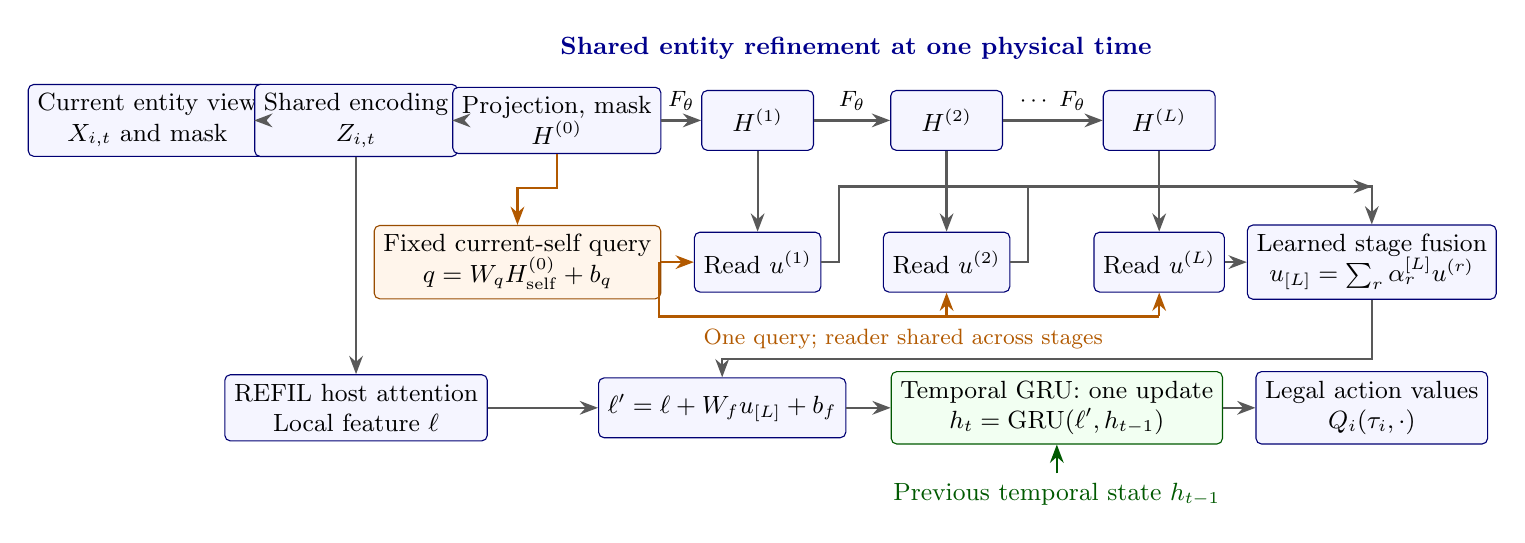
\begin{tikzpicture}[x=1cm,y=1cm,>=Stealth,
 box/.style={draw=blue!45!black,rounded corners=2pt,fill=blue!4,align=center,font=\small,minimum height=.76cm},
 smallbox/.style={box,minimum width=1.42cm},
 flow/.style={->,thick,draw=black!65},
 queryflow/.style={->,thick,draw=orange!70!black},
 every node/.style={font=\small}]
\node[box,minimum width=2.0cm] (obs) at (0,0) {Current entity view\\$X_{i,t}$ and mask};
\node[box,minimum width=1.9cm] (enc) at (2.65,0) {Shared encoding\\$Z_{i,t}$};
\node[box,minimum width=1.7cm] (h0) at (5.2,0) {Projection, mask\\$H^{(0)}$};
\node[smallbox] (h1) at (7.75,0) {$H^{(1)}$};
\node[smallbox] (h2) at (10.15,0) {$H^{(2)}$};
\node[smallbox] (hl) at (12.85,0) {$H^{(L)}$};
\draw[flow] (obs) -- (enc);
\draw[flow] (enc) -- (h0);
\draw[flow] (h0) -- node[above,font=\footnotesize] {$F_\theta$} (h1);
\draw[flow] (h1) -- node[above,font=\footnotesize] {$F_\theta$} (h2);
\draw[flow] (h2) -- node[above,font=\footnotesize] {$\cdots\ F_\theta$} (hl);
\node[font=\small\bfseries,text=blue!55!black] at (9.0,.92) {Shared entity refinement at one physical time};
\node[box,fill=orange!8,draw=orange!60!black,minimum width=2.5cm] (query) at (4.7,-1.8) {Fixed current-self query\\$q=W_qH^{(0)}_{\rm self}+b_q$};
\node[smallbox] (u1) at (7.75,-1.8) {Read $u^{(1)}$};
\node[smallbox] (u2) at (10.15,-1.8) {Read $u^{(2)}$};
\node[smallbox] (ul) at (12.85,-1.8) {Read $u^{(L)}$};
\draw[queryflow] (h0.south) -- ++(0,-.43) -| (query.north);
\draw[flow] (h1) -- (u1);
\draw[flow] (h2) -- (u2);
\draw[flow] (hl) -- (ul);
\draw[queryflow] (query.east) -- (u1.west);
\draw[draw=orange!70!black,thick] (6.5,-1.8) -- (6.5,-2.49) -- (12.85,-2.49);
\draw[queryflow] (10.15,-2.49) -- (u2.south);
\draw[queryflow] (12.85,-2.49) -- (ul.south);
\node[font=\footnotesize,text=orange!70!black] at (9.6,-2.77) {One query; reader shared across stages};
\node[box,minimum width=2.4cm] (fusion) at (15.55,-1.8) {Learned stage fusion\\$u_{[L]}=\sum_r\alpha_r^{[L]}u^{(r)}$};
\draw[flow] (ul) -- (fusion);
\draw[flow] (u1.east) -- ++(.22,0) |- (15.55,-.84) -- (fusion.north);
\draw[flow] (u2.east) -- ++(.22,0) |- (15.55,-.84);
\node[box,minimum width=2.3cm] (base) at (2.65,-3.65) {REFIL host attention\\Local feature $\ell$};
\node[box,minimum width=2.45cm] (res) at (7.3,-3.65) {$\ell'=\ell+W_f u_{[L]}+b_f$};
\node[box,fill=green!5,draw=green!35!black,minimum width=2.8cm] (gru) at (11.55,-3.65) {Temporal GRU: one update\\$h_t=\operatorname{GRU}(\ell',h_{t-1})$};
\node[box,minimum width=2.15cm] (qval) at (15.55,-3.65) {Legal action values\\$Q_i(\tau_i,\cdot)$};
\draw[flow] (enc.south) -- (base.north);
\draw[flow] (base) -- (res);
\draw[flow] (fusion.south) |- (7.3,-3.03) -- (res.north);
\draw[flow] (res) -- (gru);
\draw[flow] (gru) -- (qval);
\node[font=\small,text=green!35!black] (prev) at (11.55,-4.75) {Previous temporal state $h_{t-1}$};
\draw[flow,draw=green!35!black] (prev.north) -- (gru.south);
\end{tikzpicture}
}
\caption{LEAF at one defender decision. The same context-update operator refines the receiver-relative entity set across rounds. A fixed current-self query reads each stage, and learned fusion augments the host feature before the temporal GRU updates once. Context states are reinitialized at every physical step; only temporal memory persists. Training samples one to four rounds, formal comparison uses four, and frozen-depth analysis evaluates one to six.}
\label{fig:framework}
\end{figure*}
\section{Looped Entity Attention Fusion}
\label{sec:method}
An attacker's urgency depends on the asset it threatens and the teammates already covering that asset. LEAF develops this threat context before the acting defender reads it. We organize its computation into four modules: entity-context construction (C), current-self querying and reading (Q), intermediate-stage fusion (F), and host-feature integration with temporal decision memory (H). Shared parameters and sampled training depths determine how the context operator is learned and reused. Context processing takes place within one physical decision; the downstream GRU carries memory across decisions. Figure~\ref{fig:framework} shows these information paths, and Section~\ref{subsec:ablation} maps the trained ablations to the four modules.

\subsection{Receiver-Relative Entities and Host Features}
At time $t$, defender $i$ receives an entity matrix $X_{i,t}$. The self row retains absolute position and velocity; other rows express them relative to this defender. Features also include entity type, health, alive status, target damage, and defenders' previous actions. Let $m_{i,t,e}=1$ denote an excluded entity. Unobserved, dead, and padding entities cannot act as keys, and $\operatorname{Mask}_m$ zeros their working states. REFIL's imagined branches add their partition masks; these masks also apply to the relational path.

A shared rowwise encoder produces 128-dimensional tokens $Z_{i,t}$. Two paths use these same tokens: the REFIL host pools them with self-conditioned attention to form a 64-dimensional local feature $\ell_{i,t}$; the relational path retains the entity set,
\begin{equation}
 E_{i,t}=W_g Z_{i,t}+b_g,\qquad
 H^{(0)}_{i,t}=\operatorname{Mask}_{m_{i,t}}(E_{i,t}),
 \label{eq:workspace}
\end{equation}
with working width $d=64$. Thus contextual processing begins from individual entities, not from the already pooled host feature. All defenders share parameters but construct their own relative views. The entity states are initialized anew at each observation and receive no preceding GRU state.

\subsection{Shared Contextual Refinement}
Suppressing $i,t$, LEAF applies the same operator $F_\theta$ for $L$ rounds:
\begin{align}
 J^{(r)}&=\operatorname{LN}_a(H^{(r-1)}),\nonumber\\
 \widetilde H^{(r)}&=H^{(r-1)}+
       \operatorname{MHA}_{\theta}(J^{(r)},H^{(r-1)},H^{(r-1)};m),\nonumber\\
 H^{(r)}&=\operatorname{Mask}_{m}\!\left[\widetilde H^{(r)}+
       \operatorname{FFN}_{\theta}(\operatorname{LN}_f(\widetilde H^{(r)}))\right].
 \label{eq:loop}
\end{align}
Here layer normalization and the feedforward network act rowwise. Masked multihead attention uses four heads, and the feedforward hidden width is $2d$. Its queries use normalized states; keys and values use the preceding states directly. This combination lets an attacker token incorporate target and teammate context before a defender selects information from it. Later rounds reconsider already contextualized representations with the same transformation, following the shared-depth principle of Universal Transformers~\cite{dehghani2019universal}.

All permitted entities can interact in the first round. Increasing $r$ therefore changes the processing of a scene already globally accessible to the receiver; it does not expose a successively larger graph neighborhood. Neither the residual architecture nor parameter sharing implies convergence or monotonic improvement with depth. The benefit sought is a reusable contextual transformation, assessed through separately trained variants and frozen-depth evaluation.

\subsection{Current-State Reading and Stage Fusion}
One query, fixed throughout the current decision, reads every stage:
\begin{align}
 q_{i,t}&=W_q H^{(0)}_{i,t,\mathrm{self}}+b_q,\nonumber\\
 u_{i,t}^{(r)}&=\operatorname{MHA}_{\mathrm{read}}
          (q_{i,t},H_{i,t}^{(r)},H_{i,t}^{(r)};m_{i,t}).
 \label{eq:read}
\end{align}
This affine query uses the current self token, with the temporal-state input fixed to zero. The token obeys the relational mask, including in imagined branches. Context-update and reader parameters are distinct, and each is shared across rounds. The reader converts scene context into a receiver-specific feature without updating the query from either the loop state or temporal memory.

A shared linear scorer combines the intermediate reads:
\begin{align}
 s_r&=w_s^\top u^{(r)}+b_s,\qquad
 \alpha_r^{[L]}=\frac{\exp(s_r)}{\sum_{j=1}^{L}\exp(s_j)},\nonumber\\
 u_{[L]}&=\sum_{r=1}^{L}\alpha_r^{[L]}u^{(r)}.
 \label{eq:fusion}
\end{align}
The scorer sees only its stage's read; receiver information enters through that read. As in intermediate-representation aggregation~\cite{xu2018jk}, this preserves access to earlier features instead of requiring the final stage to carry all useful information. Entity attention selects information within a stage, whereas Eq.~\eqref{eq:fusion} weights stages. All $L$ updates are executed: the weights implement information fusion, not a stopping rule.

The host feature and fused read jointly enter the recurrent decision network,
\begin{align}
 \ell'_{i,t}&=\ell_{i,t}+W_f u_{[L],i,t}+b_f,\nonumber\\
 h_{i,t}&=\operatorname{GRU}_{\mathrm{time}}(\ell'_{i,t},h_{i,t-1}),\nonumber\\
 Q_i(\tau_{i,t},\cdot)&=W_o h_{i,t}+b_o.
 \label{eq:decision}
\end{align}
The projection $W_f,b_f$ is zero-initialized and then trained jointly with both feature paths. The 64-dimensional GRU updates once per physical decision, integrating temporal information as in recurrent value learning~\cite{hausknecht2015drqn}. The policy selects the highest-valued legal maneuver; it has no explicit defender--attacker assignment output.

This placement gives an exact, limited form of memory isolation. For fixed parameters, depth, mask, and observed features, including the previous-action features,
\begin{equation}
 \left.\frac{\partial u_{[L],i,t}}{\partial h_{i,t-1}}\right|_{X_{i,t},m_{i,t}}=0.
 \label{eq:memory-isolation}
\end{equation}
Indeed, neither initialization, contextual updates, query, nor fusion uses $h_{i,t-1}$. Action values can still depend on it through the GRU. This is a statement about the instantaneous computation, not statistical independence from history. The memory-query variant supplies a stopped-gradient $h_{i,t-1}$ to Eq.~\eqref{eq:read}; stopping its gradient does not remove its forward influence. Both policies retain temporal memory.

\subsection{Training Across Depths}
Collection samples $L$ uniformly from $\{1,2,3,4\}$ per environment and holds it fixed for an episode. Replay independently samples one depth per minibatch, used consistently by the online, target, and imagined branches. With REFIL's main and imagined temporal-difference losses~\cite{iqbal2021refil}, this optimizes
\begin{equation}
 \mathcal L=\mathbb E_L
 \left[(1-\lambda)\mathcal L_{\mathrm{TD}}^{[L]}
       +\lambda\mathcal L_{\mathrm{imagined}}^{[L]}\right],\quad\lambda=0.5.
 \label{eq:td-loss}
\end{equation}
Each sampled depth supervises a complete fused policy. The shared operator is consequently trained both on initial tokens and on its own intermediate outputs, and the scorer is trained with different available stage sets. The host's FlexQMIX mixer, imagined grouping, and value-learning protocol are retained. Training may use potential shaping; formal evaluation measures unshaped target damage, $R=-D$. Deployment uses only the main branch and no mixer.

The formal policy uses final weights and $L=4$. Frozen evaluations at $L=1$--$4$ vary depth within the training range; $L=5,6$ examine depth extrapolation. These differ from training a one-round policy or a fixed four-round policy from scratch. Parameter count is independent of population and shared unfolding depth, but dense contextual updates cost $O(L(M^2d+Md^2))$ per receiver for $M$ entity slots. Variable input size and execution depth are architectural capabilities; their protection performance requires empirical evaluation.

\subsection{Structural Properties and a Finite-Depth Bound}
We state what the architecture guarantees, separately from its empirical generalization. Consider deterministic evaluation with at least one permitted key and fixed observed features and entering temporal state.

\noindent\textbf{Proposition 1 (masked set consistency).}
Let $P$ permute entity rows while preserving the receiver's self row, with masks and all row features permuted together. At every depth, $H^{(r)}(PX,Pm)=P H^{(r)}(X,m)$, while $u_{[L]}$ and the defender's action values are unchanged.

\emph{Proof.} Rowwise encoding, normalization, and feedforward maps commute with $P$. Masked attention satisfies
\begin{equation}
 \operatorname{MHA}(PQ,PK,PV;Pm)
 =P\operatorname{MHA}(Q,K,V;m),
 \label{eq:permutation}
\end{equation}
because rowwise softmax commutes with simultaneous permutation of score rows and columns. Residual addition and masking preserve this property, giving induction over Eq.~\eqref{eq:loop}. The fixed self query is unchanged; permuting its keys and values leaves each read unchanged. Fusion, host pooling, and Eq.~\eqref{eq:decision} then preserve action values. This is the masked receiver-specific form of attention's set symmetry~\cite{lee2019settransformer}.\hfill$\square$

\noindent\textbf{Proposition 2 (prefix-fusion stability).}
Compare depths $p<L$ at the same input and entering memory. Define omitted fusion mass $\beta=\sum_{r=p+1}^{L}\alpha_r^{[L]}$ and $\Delta=\max_{p<r\leq L}\|u^{(r)}-u_{[p]}\|$. Then
\begin{equation}
 \|u_{[L]}-u_{[p]}\|\leq\beta\Delta.
 \label{eq:prefix-bound}
\end{equation}
If the downstream map in Eq.~\eqref{eq:decision} is $\kappa$-Lipschitz from the chosen read norm to the action-value infinity norm on the connecting segment, the legal greedy action is unchanged whenever its depth-$L$ action-value margin exceeds $2\kappa\beta\Delta$.

\emph{Proof.} Shared updates and scoring leave prefix reads and scores unchanged, so $\alpha_r^{[p]}=\alpha_r^{[L]}/(1-\beta)$ for $r\leq p$. Hence
$u_{[L]}-u_{[p]}=\sum_{r=p+1}^{L}\alpha_r^{[L]}(u^{(r)}-u_{[p]})$.
The triangle inequality proves Eq.~\eqref{eq:prefix-bound}. Each action value changes by at most $\kappa\beta\Delta$; a larger-than-double margin preserves the maximizer.\hfill$\square$

The second result is local to a fixed decision and conditional on the stated sensitivity bound. It connects the readout weights and frozen-depth comparisons in Section~\ref{sec:results}: small late-stage weights alone do not establish negligible action effects, since feature displacement and decision margin also matter. Neither proposition guarantees reward transfer, closed-loop trajectory agreement, or convergence at arbitrary depth.

\section{Experimental Evaluation}
\label{sec:results}
% Numerical sources: the main report Tables 1 and 3 and Section 4.11.
% Saved views: comparison and design_comparison; statistics are unchanged.
% Mechanism interventions use their runtime-matched local standards.

\newcommand{\HadMainTable}{%
\begin{table*}[!t]
\centering\footnotesize
\setlength{\tabcolsep}{5pt}
\caption{Eight-method comparison of target protection: damage $D\downarrow$, mean $\pm$ sample SD across three training seeds (Rule: scene SD). Each configuration uses 300 common scenes; configurations are equally weighted. QMIX denotes the entity-attention adaptation. Bold: lowest mean.}
\label{tab:had-main}
\begin{tabular*}{\textwidth}{@{\extracolsep{\fill}}lrrrr@{}}
\toprule
Method & ID & $K$-OOD & $N$-OOD & Joint OOD \\
\midrule
\textbf{LEAF} & $\mathbf{0.405\pm0.097}$ & $\mathbf{0.996\pm0.233}$ & $\mathbf{0.575\pm0.235}$ & $\mathbf{1.097\pm0.105}$ \\
REFIL & $0.715\pm0.049$ & $1.796\pm0.304$ & $2.209\pm0.277$ & $3.308\pm0.303$ \\
ALMA & $1.326\pm0.193$ & $3.022\pm0.344$ & $3.605\pm0.742$ & $5.375\pm1.036$ \\
TransfQMix$^{\ddagger}$ & $1.529\pm0.283$ & $3.953\pm0.495$ & $4.024\pm0.968$ & $6.630\pm1.203$ \\
DCG & $2.028\pm0.437$ & $5.839\pm1.920$ & $5.021\pm2.658$ & $8.092\pm3.909$ \\
SPECTra$^{\ddagger}$ & $2.485\pm0.209$ & $6.743\pm0.528$ & $5.049\pm0.589$ & $9.838\pm0.490$ \\
Rule$^{\dagger}$ & $1.462\pm0.717$ & $3.212\pm1.126$ & $1.545\pm0.881$ & $3.060\pm0.976$ \\
QMIX & $2.318\pm1.431$ & $5.009\pm2.497$ & $5.139\pm3.111$ & $7.415\pm3.970$ \\
\bottomrule
\end{tabular*}
\par\vspace{2pt}\parbox{\textwidth}{\footnotesize
$\dagger$ Rule has no training seeds; its SD is across the 300 scene seeds after averaging configurations within each scene. Other SDs describe variation across trained models. $\ddagger$ Updated baselines align entity inputs and sampling controls while retaining their method-specific optimizer and TD settings.}
\end{table*}}

\newcommand{\HadCoreAblationTable}{%
\begin{table*}[!t]
\centering\footnotesize
\setlength{\tabcolsep}{3pt}
\caption{Historical architecture design comparisons: damage $D\downarrow$, mean $\pm$ sample SD across three training seeds, under the formal evaluation of Table~\ref{tab:had-main}. The middle column states the principal module change. C: context constructor; Q: current-self query; F: stage fusion; H: host integration. Temporal GRU is retained by every trained variant. Bold: lowest mean.}
\label{tab:had-core-ablation}
\begin{tabular*}{\textwidth}{@{\extracolsep{\fill}}lp{0.30\textwidth}rrrr@{}}
\toprule
Variant & Module / change & ID & $K$-OOD & $N$-OOD & Joint OOD \\
\midrule
\textbf{LEAF} & Complete architecture & $\mathbf{0.405\pm0.097}$ & $\mathbf{0.996\pm0.233}$ & $\mathbf{0.575\pm0.235}$ & $\mathbf{1.097\pm0.105}$ \\
Direct read & C: bypass updates; read $H^{(0)}$ & $0.928\pm0.210$ & $1.958\pm0.457$ & $2.020\pm0.446$ & $3.196\pm0.687$ \\
Memory query & Q: add stopped-gradient history & $0.527\pm0.227$ & $1.529\pm0.734$ & $0.998\pm0.621$ & $1.946\pm1.229$ \\
Last read & F: use only the exit's final read & $0.434\pm0.083$ & $1.020\pm0.100$ & $0.652\pm0.160$ & $1.269\pm0.202$ \\
No host & H: remove REFIL attention, imagined groups, and auxiliary loss & $0.510\pm0.138$ & $1.768\pm0.621$ & $1.263\pm0.653$ & $2.319\pm0.889$ \\
\bottomrule
\end{tabular*}
\par\vspace{2pt}\parbox{\textwidth}{\footnotesize
All four historical variants use stopped-gradient history queries; LEAF uses a current-self query. Direct read, Last read, and No host therefore differ in query placement as well as the listed module. No host retains the self-projection residual and temporal memory. Depth-training and parameter-sharing comparisons appear in Table~\ref{tab:had-supplement}.}
\end{table*}}

\newcommand{\HadMechanismTable}{%
\begin{table*}[!t]
\centering\footnotesize
\setlength{\tabcolsep}{3pt}
\caption{Frozen-policy mechanism interventions: paired damage increase $\Delta D=D_{\mathrm{intervention}}-D_{\mathrm{local\ standard}}$, mean $\pm$ sample SD across three models. Each model uses ten scenes per configuration. Positive values indicate worse protection. These interventions probe learned policy dependence, not independently retrained removals.}
\label{tab:leaf-mechanism}
\begin{tabular*}{\textwidth}{@{\extracolsep{\fill}}llrrr@{}}
\toprule
Intervention & Path probed & $(10,10,2)$ & $(50,50,2)$ & $(30,30,12)$ \\
\midrule
Read initial $H^{(0)}$ & H1: constructed context & $7.556\pm1.365$ & $18.962\pm5.828$ & $32.968\pm8.447$ \\
Zero relational residual & H1: relational feature path & $5.950\pm1.525$ & $13.695\pm6.899$ & $18.788\pm1.144$ \\
Force final read & H2: intermediate-stage fusion & $6.728\pm3.186$ & $19.937\pm12.955$ & $25.558\pm16.414$ \\
Reset Temporal GRU & H2: downstream temporal memory & $1.423\pm0.760$ & $1.294\pm0.869$ & $1.655\pm2.563$ \\
\bottomrule
\end{tabular*}
\par\vspace{2pt}\parbox{\textwidth}{\footnotesize
The $H^{(0)}$ bypass uses SkyHAD 3.0.0; the other interventions use the archived HAD-workbench 2.1.0 runtime. Each difference is paired with its corresponding local standard, separately from the formal 300-scene evaluation.}
\end{table*}}

\newcommand{\HadSupplementTable}{%
\begin{table*}[!t]
\centering\footnotesize
\setlength{\tabcolsep}{3pt}
\caption{Supplementary design and capacity controls: damage $D\downarrow$, mean $\pm$ sample SD across three training seeds. Each row is separately trained with the same physical-step budget and uses the formal evaluation of Table~\ref{tab:had-main}. These controls examine training depth, parameter sharing, and host capacity; they are distinct from the frozen exits in Fig.~\ref{fig:mechanism}(c). Bold: lowest mean.}
\label{tab:had-supplement}
\begin{tabular*}{\textwidth}{@{\extracolsep{\fill}}lp{0.30\textwidth}rrrr@{}}
\toprule
Method / variant & Design or capacity change & ID & $K$-OOD & $N$-OOD & Joint OOD \\
\midrule
\textbf{LEAF} & Shared updates; train R1--R4 & $\mathbf{0.405\pm0.097}$ & $\mathbf{0.996\pm0.233}$ & $0.575\pm0.235$ & $\mathbf{1.097\pm0.105}$ \\
One round & Train and execute R1 only & $0.609\pm0.272$ & $1.203\pm0.402$ & $1.355\pm0.884$ & $2.157\pm1.006$ \\
Fixed depth & Train at R4 throughout & $0.407\pm0.204$ & $1.004\pm0.665$ & $0.659\pm0.184$ & $1.265\pm0.230$ \\
Unshared rounds & Independent update blocks per round & $0.476\pm0.183$ & $1.127\pm0.157$ & $\mathbf{0.543\pm0.156}$ & $1.232\pm0.253$ \\
REFIL-matched & Enlarge host to 176,393 actor parameters & $0.914\pm0.165$ & $2.493\pm0.280$ & $2.269\pm0.312$ & $4.170\pm0.760$ \\
\bottomrule
\end{tabular*}
\par\vspace{2pt}\parbox{\textwidth}{\footnotesize
One round, Fixed depth, and Unshared rounds retain stopped-gradient history queries, unlike LEAF. Single-round fusion is trivial. Unshared rounds also increases parameter count. The comparisons with LEAF are not single-factor changes, and equal physical-step budgets do not imply equal computation budgets.}
\end{table*}}


\noindent\textbf{Setup.}
We evaluate the planar HAD target-protection task~\cite{skyhad2026}, using public entity-state observations, a fixed reactive--rush attacker, and at most 100 physical steps per episode. Training independently samples balanced teams $N_R=N_B=N\in\{4,6,8,10\}$ and target counts $K\in\{1,2,3\}$. Each learned method uses three training seeds and $10^6$ physical environment steps per seed. LEAF uses width 64, four attention heads, learning rate $5\times10^{-4}$, discount 0.99, batch size 32, and replay capacity 5000. It samples R1--R4 during training and uses R4 for the formal comparison. All evaluations use the final budget-complete checkpoints with frozen parameters.

In-distribution (ID) evaluation contains $(4,4,2)$, $(6,6,2)$, $(8,8,2)$, and $(10,10,3)$. Target-count extrapolation ($K$-OOD) uses $(10,10,K)$ with $K=4,6,9,12$. Team-size extrapolation ($N$-OOD) uses $(N,N,2)$ with $N=15,20,25,30,40,50$. Joint OOD combines $N=15,20,30$ with $K=4,6$, and adds $(30,30,9)$ and $(30,30,12)$. Two extra configurations, $(5,5,2)$ and $(10,10,2)$, complete the 24-configuration matrix. Every configuration uses 300 common initial scenes, seeds 9000--9299. Transfer is zero-shot: neither the policy parameters nor the entity encoder are adapted to these deployment populations. The label R1 denotes execution depth $L=1$, and similarly for the other exits.

\noindent\textbf{Metrics and uncertainty.}
The primary metric is cumulative target damage $D\downarrow$, with unshaped episode reward $R=-D$. Damage is not capped by initial target health and is not a win rate. Where recorded, we also report friendly-collision mortality $C$ (defenders killed by friendly collisions divided by initial $N_R$), attacker interception $I$, and the fraction of episodes with any target damage $P$. The updated SPECTra and TransfQMix final evaluations record damage but not these protection diagnostics. Results first average scenes within each trained model and configuration, then weight group configurations equally. The reported mean $\pm$ sample SD describes variation across three trained models~\cite{agarwal2021rliable}; Rule instead uses scene-seed SD. Validation has 50 checkpoints, each evaluating four ID configurations on 25 fixed scenes distinct from the formal pool. Curves align checkpoint indices, use actual mean environment-step counts, and show unsmoothed model means and sample SD.

\subsection{Comparison Across Deployment Populations}
\label{subsec:comparison}
The comparison in Table~\ref{tab:had-main} and Fig.~\ref{fig:comparison} includes LEAF, REFIL~\cite{iqbal2021refil}, ALMA~\cite{iqbal2022alma}, TransfQMix~\cite{transfqmix2023}, DCG~\cite{boehmer2020dcg}, SPECTra~\cite{park2026spectra}, Rule, and QMIX~\cite{rashid2018qmix}. Here QMIX denotes the documented entity-attention adaptation. The updated SPECTra and TransfQMix runs use 19-dimensional entity inputs, including the previous action, consistently in actor and mixer; both use eight parallel collectors and eight learner updates per collection. Their own optimizer and TD settings are retained: Adam at $10^{-3}$, TD($\lambda$) with $\lambda=0.6$, and half-MSE loss. All learned methods use equal physical-step budgets. This aligns inputs and sampling controls, not every training hyperparameter; the historical LEAF design comparisons provide closer architectural contrasts, with query differences noted below.

LEAF has the lowest group mean damage in all four groups. Relative to REFIL, $D$ decreases by 0.310, 0.800, 1.635, and 2.211 in ID, $K$-OOD, $N$-OOD, and Joint OOD; all three training-seed comparisons favor LEAF in each group. The larger differences when teams and targets grow together support the intended use of attacker--target--teammate context: a policy learned in small engagements continues to protect assets as the entity set expands.

Figure~\ref{fig:comparison} connects validation to deployment for the same eight methods. At checkpoint 10, around 0.2M physical steps, LEAF's validation damage is $2.046\pm0.028$, versus REFIL's $4.429\pm0.284$; the final values are $0.373\pm0.066$ and $0.738\pm0.122$. These observations describe the fixed ID validation pool, while the extrapolation panels track the frozen policies as population size changes.

Among learned comparators with recorded final protection diagnostics, LEAF has lower mean friendly-collision mortality in all four groups. This comparison excludes the updated SPECTra and TransfQMix runs. Rule has lower $C$ in $N$-OOD and Joint OOD: $5.70\pm3.30\%$ and $4.48\pm2.44\%$, compared with LEAF's $6.29\pm1.32\%$ and $4.97\pm1.26\%$. Its target damage is higher in both groups. Conserving defenders and protecting targets therefore remain distinct outcomes; the latter is the primary objective.

\HadMainTable

\begin{figure*}[!t]
\centering
\includegraphics[width=\textwidth]{../Open-SCORE/outputs/main/had/figures/fig_comparison.pdf}
\caption{Eight-method comparison of learning and zero-shot population transfer: LEAF, REFIL, ALMA, TransfQMix, DCG, SPECTra, Rule, and QMIX (the entity-attention adaptation). SPECTra and TransfQMix use the updated input/sampling protocol described in the text. (a) ID validation damage over training. (b)--(c) Frozen-policy damage under target-count and team-size extrapolation. (d) Joint-extrapolation damage. (e) Formal and independent-confirmation All24 damage; LEAF uses the separately recorded depth/confirmation reference pool and does not replace (a)--(d). Learned-method bands show one sample SD across three models; Rule is a formal reference. Table~\ref{tab:had-main} gives the group means and SDs.}
\label{fig:comparison}
\end{figure*}

\subsection{Architecture Design Comparisons}
\label{subsec:ablation}
We decompose LEAF into a context constructor (C), current-self query and reader (Q), stage fusion (F), and host integration with temporal memory (H). Table~\ref{tab:had-core-ablation} maps each historical trained variant to its principal module change; Fig.~\ref{fig:ablation} shows learning and population transfer for LEAF and all seven saved design variants. Saved configurations show that Direct read, Last read, and No host also retain the stopped-gradient history query used by Memory query, whereas LEAF uses a current-self query. They are historical design comparisons, not single-factor ablations of LEAF. Depth-training and parameter-sharing choices are analyzed separately in Section~\ref{subsec:supplement}.

\noindent\textbf{C: context construction before reading.}
\emph{Direct read} bypasses entity updates and reads $H^{(0)}$. Its damage rises from LEAF's $0.405\pm0.097$ to $0.928\pm0.210$ in ID, and from $1.097\pm0.105$ to $3.196\pm0.687$ in Joint OOD, with higher means in the other two groups as well. This trained comparison favors LEAF's combined context-construction and current-self-reading design; its query difference prevents attributing the entire gap to context construction alone. The frozen context interventions below provide complementary evidence of the trained policy's dependence on context.

\noindent\textbf{Q: current-state query with history downstream.}
\emph{Memory query} adds the stopped-gradient previous Temporal GRU hidden state to the query; it retains the reader and temporal network. LEAF's current-self query has lower group mean damage by 0.122, 0.533, 0.424, and 0.849, with three seed pairs favoring LEAF in ID and two in each OOD group. The archived seed-1 pair used six versus twelve parallel collectors (the other runs used twelve), limiting strict attribution to query placement. The result favors the chosen division of information: read the current context, then combine it with temporal history for action selection.

\noindent\textbf{F: access to intermediate stages.}
\emph{Last read} replaces stage fusion with the exit's final read. Its group means are close to LEAF, ranging from $0.434$ versus $0.405$ in ID to $1.269$ versus $1.097$ in Joint OOD. This modest retrained gap, with query history also differing, does not establish an independent benefit from fusion. It is distinct from forcing an already trained LEAF policy to use its last read, which probes dependence on the learned representation in Section~\ref{subsec:mechanism}.

\noindent\textbf{H: integration with cooperative value learning.}
\emph{No host} removes the REFIL attention path, imagined groups, and associated auxiliary loss while retaining a self-projection residual, the relational path, and Temporal GRU. LEAF has lower damage in all four groups, with the largest mean difference, 1.222, in Joint OOD. The removed host package and retained history query prevent assigning this difference to one attention layer or one loss. Temporal memory is retained by every trained variant; its deployment-time role is examined by a frozen reset intervention below.

\HadCoreAblationTable

\begin{figure*}[!t]
\centering
\includegraphics[width=\textwidth]{../Open-SCORE/outputs/main/had/figures/fig_ablation.pdf}
\caption{LEAF and seven saved design variants. (a) ID validation damage over training. (b)--(c) Frozen-policy target-count and team-size transfer. (d) Joint-extrapolation damage. Learned-method bands show one sample SD across three models. The variants retain stopped-gradient history queries, so the contrasts with LEAF are not all single-factor changes. Table~\ref{tab:had-core-ablation} and Table~\ref{tab:had-supplement} give absolute group means and sample SDs.}
\label{fig:ablation}
\end{figure*}

\subsection{Mechanism of Context Use and Reusable Refinement}
\label{subsec:mechanism}
The mechanism study tests three hypotheses implied by the architecture: the trained policy uses constructed current-scene context (H1); receiver-specific intermediate reading works with downstream temporal history (H2); and the learned refinement can be reused across execution depths (H3). The final protection metrics connect these computational observations to the task outcome.

\noindent\textbf{H1: constructed context contributes to the deployed policy.}
Table~\ref{tab:leaf-mechanism} and Fig.~\ref{fig:mechanism}(a) use existing frozen interventions on ten common scenes for each of three models and configurations $(10,10,2)$, $(50,50,2)$, and $(30,30,12)$. Reading the initial $H^{(0)}$ instead of contextualized entities worsens damage in all nine model--configuration pairs. Zeroing the complete relational residual also worsens all nine pairs. In the largest target configuration, their mean damage increases are $32.968\pm8.447$ and $18.788\pm1.144$, respectively. These interventions show that the trained policy uses both contextual processing and its relational feature path. They do not predict how a policy retrained after removal would perform. Each intervention is paired with its runtime-matched local standard, separately from the formal 300-scene pool.

\HadMechanismTable

\begin{figure*}[!t]
\centering
\includegraphics[width=\textwidth]{../Open-SCORE/outputs/main/had/figures/fig_mechanism.pdf}
\caption{Mechanism evidence aligned with the architectural hypotheses. (a) Paired damage changes for eight frozen interventions, including context bypass and zeroing the relational residual. (b) H2: normal R4 fusion weights and receiver/time variation; stacked bars show mean weights. (c) H3: frozen R1--R6 damage; shading marks depths beyond training. Hollow markers give separately trained One round references for $N$-OOD and Joint OOD, with SDs in Table~\ref{tab:had-supplement}. (d) Same-state action-change percentages for the eight interventions; diagnostic actions are not executed and use the same entering temporal state. Error bars/bands show sample SD across three model means. Each panel retains its recorded evaluation pool; Table~\ref{tab:leaf-mechanism} also reports final-read and temporal-reset interventions.}
\label{fig:mechanism}
\end{figure*}

\noindent\textbf{H2: stage reading is receiver-specific, with memory retained downstream.}
Normal R4 records contain 90 episodes and 38,693 live-defender decisions. Three models each execute ten scenes in three configurations: 10v10 with two targets, and 30v30 with two or twelve targets. The first two reads receive $98.909\pm0.265\%$, $98.755\pm0.542\%$, and $98.839\pm0.157\%$ of fusion weight, respectively (Fig.~\ref{fig:mechanism}(b)). Within a physical state, the average SD of the first-round weight across active receivers is 11.44, 13.91, and 12.68 percentage points. Its mean absolute change for the same defender at adjacent steps is 5.49, 5.34, and 5.36 points. Thus receivers sharing an engagement use the stages differently, and those choices evolve over physical time.

Forcing the final read instead of learned fusion worsens all nine model--configuration pairs in Table~\ref{tab:leaf-mechanism}; resetting Temporal GRU every physical step worsens eight of nine. These observations support the division between current-context reading and downstream history in the frozen policy; they do not measure retrained component gains. The roughly 1\% mean omitted fusion mass beyond the two-round prefix is only one factor in Proposition~2. Equation~\eqref{eq:prefix-bound} also involves read displacement; action preservation further depends on downstream sensitivity and the action-value margin. Fusion weights alone are neither causal reward contributions nor a stopping rule; normal R4 computes all four stages.

\noindent\textbf{H3: refinement is reusable across execution depths.}
Figure~\ref{fig:mechanism}(c) executes the same three final LEAF models at R1--R6 on all 24 configurations, with 300 scenes per configuration and exit. R1--R4 are within the training range; R5/R6 extend inference depth without retraining. All24 damage changes from $0.8022\pm0.1849$ at R1 to $0.7845\pm0.0434$ at R4; R5 and R6 remain close, at $0.7851\pm0.0425$ and $0.7849\pm0.0423$. The small paired R2--R4 reduction, 0.008249, has a three-seed 95\% $t$ interval of $[-0.008362,0.024859]$. This is a separately recorded depth-evaluation pool; its R4 values do not replace Table~\ref{tab:had-main}.

The frozen R1 group means in ID, $N$-OOD, and Joint OOD (0.4194, 0.6086, 1.0968) are also below those of the separately trained One round model (0.609, 1.355, 2.157; Table~\ref{tab:had-supplement}). This descriptive, cross-pool comparison shows that useful short execution is compatible with multi-depth training, and the observed advantage does not require executing several rounds at deployment. The One round model also retains a history query; this is not a scene-paired contrast, a single-factor depth-training contrast, or a comparison of equal training computation.

Depth ordering still depends on the configuration. At $(30,30,12)$, R1 has mean damage 1.6378 versus R4's 2.1674; at $(30,30,2)$, R4 has 0.5370 versus R1's 0.6426. Changing depth also changes the reads available to fusion and, through later actions, the temporal states. These closed-loop results support reuse over the evaluated range, not monotonic improvement or arbitrary-depth convergence.



\HadSupplementTable

\begin{figure*}[!t]
\centering
\includegraphics[width=\textwidth]{../Open-SCORE/outputs/main/had/figures/fig_protection.pdf}
\caption{Formal team protection on 300 scenes per configuration. Collision mortality $C$, attacker interception $I$, and target-damage incidence $P$ retain their recorded model-seed means and sample SDs. The first-damage cumulative incidence includes undamaged episodes as non-events rather than dropping them. These formal outcomes are separate from the local frozen and same-state diagnostics in Fig.~\ref{fig:mechanism}.}
\label{fig:protection}
\end{figure*}

\noindent\textbf{From context use to team protection.}
The formal outcomes in Fig.~\ref{fig:protection} return to all 300 scenes per configuration. At $(10,10,2)$, LEAF intercepts $86.38\pm2.31\%$ of attackers versus REFIL's $77.00\pm2.32\%$, while damage incidence falls from $55.22\pm3.10\%$ to $30.44\pm6.74\%$. The same direction holds at $(30,30,2)$ and $(30,30,12)$, despite the different numbers of threatened assets. At $(50,50,2)$, LEAF raises interception to $78.68\pm1.39\%$ from $72.27\pm0.77\%$, reduces collision mortality to $11.14\pm2.63\%$ from $19.59\pm3.69\%$, and reduces damage incidence to $28.11\pm15.03\%$ from $70.56\pm7.65\%$. The representation and recurrent controller thus produce measurable team protection beyond the small training populations.

\subsection{Supplementary Analysis}
\label{subsec:supplement}
The supporting controls in Table~\ref{tab:had-supplement} examine capacity and refinement choices without treating them as additional representation modules.

\noindent\textbf{Capacity control.}
REFIL-matched has 176,393 actor parameters, close to LEAF's 175,754; standard REFIL has 102,025. LEAF retains lower mean damage in all four groups. A comparable parameter budget for the host therefore does not reproduce the protection results, although parameter matching does not establish equal compute cost.

\noindent\textbf{Training depth and parameter sharing.}
\emph{One round} is trained from scratch and executed at R1. Relative to Direct read within the history-query family, one contextual update reduces group mean damage by 0.319, 0.755, 0.665, and 1.039; two of three seed comparisons improve in every group. LEAF further lowers the group means, but that comparison jointly changes query history, depth training, and access to intermediate reads. One round is locally better at $(10,10,12)$, with $D=1.548\pm0.439$ versus LEAF's $1.625\pm0.515$. \emph{Fixed depth} trains at R4 throughout and has group means close to LEAF. \emph{Unshared rounds} uses independent context-update blocks, increasing parameter count, and has lower mean $N$-OOD damage (0.543 versus 0.575). Both also retain history queries. These historical controls characterize design choices; they do not establish a universal independent gain from depth sampling or sharing.


\noindent\textbf{Independent scene confirmation.}
An independent pool of 300 scenes per configuration reuses the frozen models under the archived matched HAD-workbench protocol. All24 damage is $0.7901\pm0.0395$ for LEAF R4, $2.0857\pm0.1905$ for REFIL, $4.2549\pm0.7413$ for the updated TransfQMix, and $6.2964\pm0.0723$ for the updated SPECTra. This corroborates the protection ordering on another scene pool without selecting a new depth. Historical 10-dimensional baseline runs remain archived separately from the updated runs and are not pooled into these means.

\FloatBarrier
\section{Conclusion}
LEAF treats zero-shot multi-target defense as a problem of constructing reusable threat context. A shared attention operator refines current entities, a current-self query reads the intermediate stages, and learned fusion supplies the resulting feature to downstream temporal memory. This separates within-decision scene processing from inference across physical time.

Across the evaluated SkyHAD populations, LEAF achieves lower mean target damage than the learned baselines and Rule. Historical design comparisons favor current-state reading, while frozen interventions show dependence on constructed context; the effects of sharing, fixed-depth training, and fusion remain configuration-dependent. Frozen execution remains effective over one to six rounds, while normal reads emphasize early context. Higher interception and lower target-damage incidence connect these representations to the intended protection outcome. The structural propositions explain permutation consistency and sufficient local action stability; population transfer and closed-loop depth robustness remain empirical findings within the tested setting.

\section*{Acknowledgment}
OpenAI Codex assisted with manuscript drafting and figure preparation. The conceptual illustration in Fig.~\ref{fig:motivation} was generated with ImageGen; experimental plots use the recorded results.
\bibliographystyle{IEEEtran}
\IEEEtriggeratref{19}
\bibliography{references}
\end{document}
